\documentclass[a4paper,10pt,landscape,twocolumn]{scrartcl}

%% Settings
\newcommand\problemset{3}
\newcommand\deadline{Thursday, 14 September 2017, 20:00h}
\newif\ifcomments
\commentsfalse % hide comments
%\commentstrue % show comments

%% Packages
\usepackage[english]{exercises}
\usepackage{wasysym}
\usepackage{graphicx}
\usepackage{hyperref}
\hypersetup{colorlinks=true, urlcolor = blue, linkcolor = blue}

%% Macros
\usepackage{xspace}

\newcommand{\eps}{\varepsilon}
\newcommand{\ket}[1]{|#1\rangle}
\newcommand{\bra}[1]{\langle#1|}
\newcommand{\inp}[2]{\langle{#1}|{#2}\rangle}
\newcommand{\norm}[1]{\parallel\!#1\!\parallel}
\newcommand{\points}[1]{\marginpar{\textbb{#1 p.}}}
\newtheorem{theorem}{Theorem}
\newtheorem{definition}{Definition}
\newtheorem{proposition}{Proposition}
%\newenvironment{proof}{\noindent {\bf Proof }}{{\hfill $\Box$}\\}

\newcommand{\gen}{\ensuremath{\mathsf{Gen}}\xspace}
\newcommand{\enc}{\ensuremath{\mathsf{Enc}}\xspace}
\newcommand{\dec}{\ensuremath{\mathsf{Dec}}\xspace}
\newcommand{\mac}{\ensuremath{\mathsf{Mac}}\xspace}
\newcommand{\vrfy}{\ensuremath{\mathsf{Vrfy}}\xspace}
\newcommand{\negl}{\ensuremath{\mathsf{negl}}\xspace}
\newcommand{\PrivK}{\ensuremath{\mathsf{PrivK}}\xspace}
\newcommand{\eav}{\ensuremath{\mathsf{eav}}\xspace}

\newcommand{\Z}{\ensuremath{\mathbb{Z}}}
\newcommand{\R}{\ensuremath{\mathbb{R}}}
\newcommand{\N}{\ensuremath{\mathbb{N}}}


\newcommand\floor[1]{\lfloor#1\rfloor}
\newcommand\ceil[1]{\lceil#1\rceil}

% \newcommand{\comment}[1]{{\sf [#1]}\marginpar[\hfill !!!]{!!!}}
\newcommand{\chris}[1]{\comment{\color{blue}Chris: #1}}
\newcommand{\jan}[1]{\comment{\color{magenta}Jan: #1}}


\begin{document}

\problems

{\sffamily\noindent
We will work on the following exercises together during the work sessions on Tuesday. 

The last questions are marked as homework exercises. 
Your homework must be handed in within one week \textbf{electronically via Canvas before \deadline}. This deadline is strict and late submissions are graded with a 0. At the end of the course, the lowest of all the homework grades will be dropped. 

You are strongly encouraged to work together on the exercises, including the homework. However, after this discussion phase, you have to write down and submit your own individual solution. }

\begin{exercise}[Insecurity of Multi-Time Pad]
Two ASCII messages containing English letters and spaces only are encrypted using the one-time pad and the same key. The 10th byte of the first ciphertext is observed to be \texttt{0xB7} and the 10th byte of the second ciphertext is observed to be \texttt{0xE7}. Let $m_1$ (resp., $m_2$) denote the 10th ASCII character in the first (resp., second) message. What is the most you can conclude about $m_1$ and $m_2$?
\end{exercise}

\begin{figure}[h]
\center
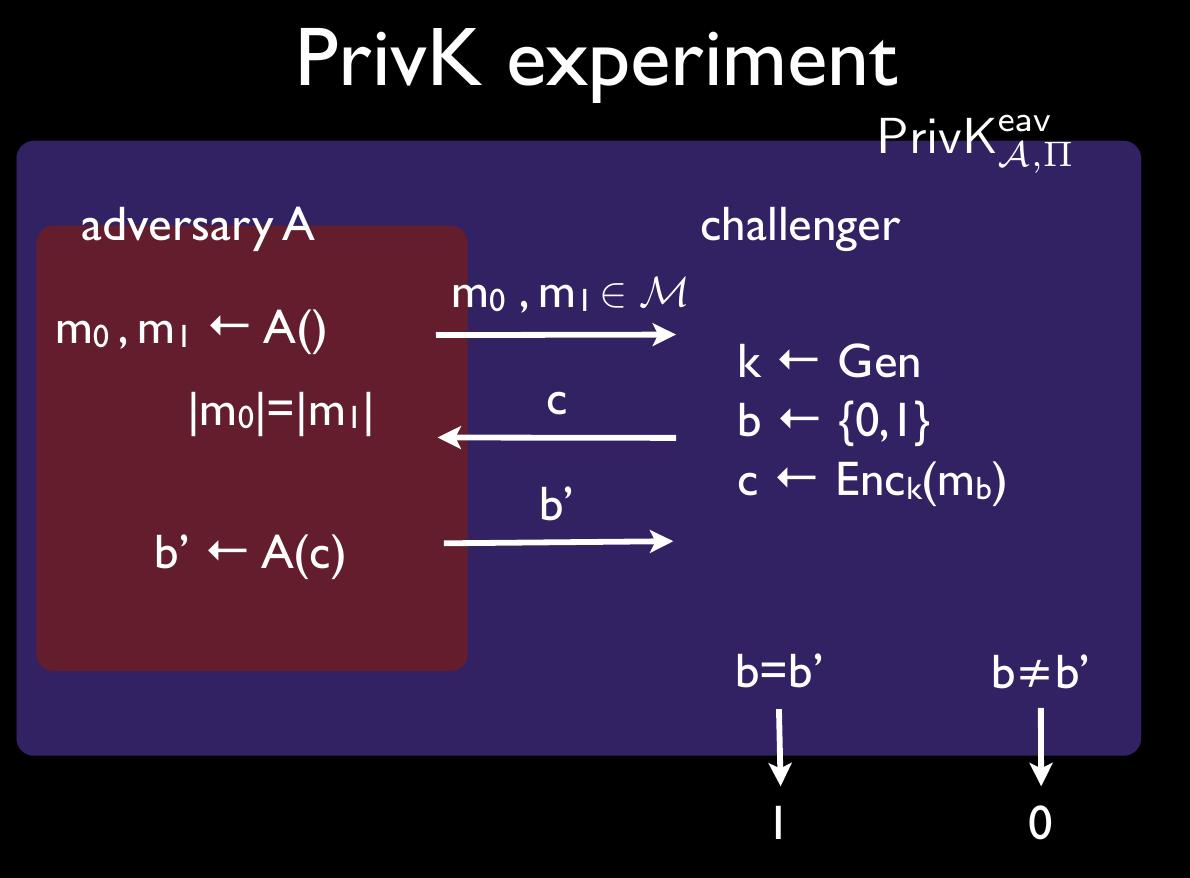
\includegraphics[width=8cm]{PrivKexperiment.jpg}
\caption{The $\PrivK^{\eav}_{\mathcal{A},\Pi}$ experiment \label{fig}}
\end{figure}

\begin{exercise}[The $\PrivK^{\eav}_{\mathcal{A},\Pi}$ experiment (see Figure~\ref{fig})]
For each of the following scenarios, give the maximal value of $\Pr[\PrivK^{\eav}_{\mathcal{A},\Pi}=1]$ and explain how it can be achieved.

\begin{subex}
Let $\Pi$ be the shift cipher, and let us consider an adversary $\mathcal{A}$ that submits $m_0 = \mathtt{a}$ and $m_1 = \mathtt{a}$. 
\end{subex}

\begin{subex}
Let $\Pi$ be the shift cipher, and let us consider an adversary $\mathcal{A}$ that submits $m_0 = \mathtt{a}$ and $m_1 = \mathtt{b}$. 
\end{subex}

\begin{subex}
Let $\Pi$ be the shift cipher, and let us consider an adversary $\mathcal{A}$ that submits $m_0 = \mathtt{aa}$ and $m_1 = \mathtt{bb}$. 
\end{subex}

\begin{subex}
Let $\Pi$ be the shift cipher, and let us consider an adversary $\mathcal{A}$ that submits $m_0 = \mathtt{aa}$ and $m_1 = \mathtt{ab}$. 
\end{subex}

\begin{subex}
Let $\Pi$ be the one-time-pad encryption, and let us consider an adversary $\mathcal{A}$ that submits $m_0 = \mathtt{aaa}$ and $m_1 = \mathtt{abc}$. 
\end{subex}

\begin{subex}
Let $\Pi$ be the monoalphabetic substitution cipher. Give an adversary $\mathcal{A}$ that manages to win the $\PrivK^{\eav}_{\mathcal{A},\Pi}$ experiment all the time, i.e.\ such that $\Pr[\PrivK^{\eav}_{\mathcal{A},\Pi}=1] = 1$.
\end{subex}
\end{exercise}


\begin{exercise}[Exercise~3.1 from  $\text{[KL]}$ ]
Prove Proposition 3.6:
Let $\negl_1$ and $\negl_2$ be negligible functions. Then,
\begin{enumerate}
\item The function $\negl_3$ defined by $\negl_3(n) = \negl_1(n)+\negl_2(n)$ is
  negligible.
\item For any positive polynomial $p$, the function $\negl_4$ defined
  by $\negl_4(n) = p(n) \cdot \negl_1(n)$ is negligible.
\end{enumerate}
\end{exercise}

\begin{exercise}[Exercise~3.2 from $\text{[KL]}$ ]
Prove that Definition~3.8 cannot be
  satisfied if $\Pi$ can encrypt arbitrary-length messages and the
  adversary is not restricted to output equal-length messages in
  experiment $\PrivK^{\eav}_{\mathcal{A},\Pi}$. \textbf{ Hint:} Let $q(n)$
  be a polynomial upper-bound on the length of the cipher-text when
  $\Pi$ is used to encrypt a single bit. Then consider an adversary
  who outputs $m_0 \in \{0, 1\}$ and a uniform $m_1 \in \{0, 1\}^{q(n)+2}$.
\end{exercise}

\begin{exercise}[Exercise~3.3 from  $\text{[KL]}$ ]
Say $\Pi=\left( \gen,\enc,\dec \right)$ is such that for $k\in \{0,1\}^n$, algorithm $\enc_k$ is only defined for messages of length at most $\ell(n)$ (for some polynomial $\ell$). Construct a scheme satisfying Definition~3.8 even when the adversary is \emph{not} restricted to outputting equal-length messages in $\PrivK^{\eav}_{\mathcal{A},\Pi}$. 

  
\end{exercise}

\begin{exercise}[Exercise~3.4 from  $\text{[KL]}$ ]
Prove the equivalence of Definition 3.8 and Definition 3.9 from the book [KL].
\end{exercise}
  


\end{document}
